\documentclass[twoside]{book}

% Packages required by doxygen
\usepackage{fixltx2e}
\usepackage{calc}
\usepackage{doxygen}
\usepackage[export]{adjustbox} % also loads graphicx
\usepackage{graphicx}
\usepackage[utf8]{inputenc}
\usepackage{makeidx}
\usepackage{multicol}
\usepackage{multirow}
\PassOptionsToPackage{warn}{textcomp}
\usepackage{textcomp}
\usepackage[nointegrals]{wasysym}
\usepackage[table]{xcolor}

% Font selection
\usepackage[T1]{fontenc}
\usepackage[scaled=.90]{helvet}
\usepackage{courier}
\usepackage{amssymb}
\usepackage{sectsty}
\renewcommand{\familydefault}{\sfdefault}
\allsectionsfont{%
  \fontseries{bc}\selectfont%
  \color{darkgray}%
}
\renewcommand{\DoxyLabelFont}{%
  \fontseries{bc}\selectfont%
  \color{darkgray}%
}
\newcommand{\+}{\discretionary{\mbox{\scriptsize$\hookleftarrow$}}{}{}}

% Page & text layout
\usepackage{geometry}
\geometry{%
  a4paper,%
  top=2.5cm,%
  bottom=2.5cm,%
  left=2.5cm,%
  right=2.5cm%
}
\tolerance=750
\hfuzz=15pt
\hbadness=750
\setlength{\emergencystretch}{15pt}
\setlength{\parindent}{0cm}
\setlength{\parskip}{3ex plus 2ex minus 2ex}
\makeatletter
\renewcommand{\paragraph}{%
  \@startsection{paragraph}{4}{0ex}{-1.0ex}{1.0ex}{%
    \normalfont\normalsize\bfseries\SS@parafont%
  }%
}
\renewcommand{\subparagraph}{%
  \@startsection{subparagraph}{5}{0ex}{-1.0ex}{1.0ex}{%
    \normalfont\normalsize\bfseries\SS@subparafont%
  }%
}
\makeatother

% Headers & footers
\usepackage{fancyhdr}
\pagestyle{fancyplain}
\fancyhead[LE]{\fancyplain{}{\bfseries\thepage}}
\fancyhead[CE]{\fancyplain{}{}}
\fancyhead[RE]{\fancyplain{}{\bfseries\leftmark}}
\fancyhead[LO]{\fancyplain{}{\bfseries\rightmark}}
\fancyhead[CO]{\fancyplain{}{}}
\fancyhead[RO]{\fancyplain{}{\bfseries\thepage}}
\fancyfoot[LE]{\fancyplain{}{}}
\fancyfoot[CE]{\fancyplain{}{}}
\fancyfoot[RE]{\fancyplain{}{\bfseries\scriptsize Generated by Doxygen }}
\fancyfoot[LO]{\fancyplain{}{\bfseries\scriptsize Generated by Doxygen }}
\fancyfoot[CO]{\fancyplain{}{}}
\fancyfoot[RO]{\fancyplain{}{}}
\renewcommand{\footrulewidth}{0.4pt}
\renewcommand{\chaptermark}[1]{%
  \markboth{#1}{}%
}
\renewcommand{\sectionmark}[1]{%
  \markright{\thesection\ #1}%
}

% Indices & bibliography
\usepackage{natbib}
\usepackage[titles]{tocloft}
\setcounter{tocdepth}{3}
\setcounter{secnumdepth}{5}
\makeindex

% Hyperlinks (required, but should be loaded last)
\usepackage{ifpdf}
\ifpdf
  \usepackage[pdftex,pagebackref=true]{hyperref}
\else
  \usepackage[ps2pdf,pagebackref=true]{hyperref}
\fi
\hypersetup{%
  colorlinks=true,%
  linkcolor=blue,%
  citecolor=blue,%
  unicode%
}

% Custom commands
\newcommand{\clearemptydoublepage}{%
  \newpage{\pagestyle{empty}\cleardoublepage}%
}

\usepackage{caption}
\captionsetup{labelsep=space,justification=centering,font={bf},singlelinecheck=off,skip=4pt,position=top}

%===== C O N T E N T S =====

\begin{document}

% Titlepage & ToC
\hypersetup{pageanchor=false,
             bookmarksnumbered=true,
             pdfencoding=unicode
            }
\pagenumbering{roman}
\begin{titlepage}
\vspace*{7cm}
\begin{center}%
{\Large pruner \\[1ex]\large 0.\+0-\/99 }\\
\vspace*{1cm}
{\large Generated by Doxygen 1.8.11}\\
\end{center}
\end{titlepage}
\clearemptydoublepage
\tableofcontents
\clearemptydoublepage
\pagenumbering{arabic}
\hypersetup{pageanchor=true}

%--- Begin generated contents ---
\chapter{Main Page}
\label{index}\hypertarget{index}{}\href{https://travis-ci.org/USCbiostats/pruner}{\tt }

\section*{pruner\+: Implementing the Felsenstein\textquotesingle{}s \hyperlink{classTree}{Tree} Pruning algorithm}

This C++ template library provides classes to implement Felsenstein tree-\/pruning algorithm for efficiently computing likelihood functions on phylogenies.

The library reads in a tree object in the form of {\ttfamily std\+::vector$<$ unsigned int $>$} specifying the source and target of each dyad (edge) and allows the user to store arbitrary arguments using memory pointers, and {\ttfamily std\+::function} to be called with those arbitrary arguments and tree structure data.

Trees are stored as two lists\+: each nodes\textquotesingle{} offspring, and each nodes\textquotesingle{} parents, which can be accessed at any point using {\ttfamily \hyperlink{classTreeIterator}{Tree\+Iterator}} class that implements tree traversals (pre and post order for pruning).

\subsection*{Contributing}

We welcome contributions to {\ttfamily pruner}. Whether it is reporting a bug, starting a discussion by asking a question, or proposing/requesting a new feature, please go by creating a new issue \href{https://github.com/USCbiostats/pruner/issues}{\tt here} so that we can talk about it.

Please note that this project is released with a https\+://github.com/\+U\+S\+Cbiostats/pruner/blob/master/\+C\+O\+D\+E\+\_\+\+O\+F\+\_\+\+C\+O\+N\+D\+U\+C\+T.\+md \char`\"{}\+Contributor Code of Conduct\char`\"{}. By participating in this project you agree to abide by its terms.

\subsection*{Funding}

Supported by National Cancer Institute Grant \#1\+P01\+C\+A196596. 
\chapter{Class Index}
\section{Class List}
Here are the classes, structs, unions and interfaces with brief descriptions\+:\begin{DoxyCompactList}
\item\contentsline{section}{\hyperlink{classpruner_1_1Tree}{pruner\+::\+Tree$<$ Data\+\_\+\+Type $>$} \\*\hyperlink{classpruner_1_1Tree}{Tree} class }{\pageref{classpruner_1_1Tree}}{}
\item\contentsline{section}{\hyperlink{classTree}{Tree$<$ Data\+\_\+\+Type $>$} \\*\hyperlink{classTree}{Tree} class }{\pageref{classTree}}{}
\item\contentsline{section}{\hyperlink{classTreeIterator}{Tree\+Iterator$<$ Data\+\_\+\+Type $>$} }{\pageref{classTreeIterator}}{}
\item\contentsline{section}{\hyperlink{classpruner_1_1TreeIterator}{pruner\+::\+Tree\+Iterator$<$ Data\+\_\+\+Type $>$} }{\pageref{classpruner_1_1TreeIterator}}{}
\end{DoxyCompactList}

\chapter{File Index}
\section{File List}
Here is a list of all documented files with brief descriptions\+:\begin{DoxyCompactList}
\item\contentsline{section}{include/{\bfseries pruner.\+h} }{\pageref{pruner_8h}}{}
\item\contentsline{section}{include/{\bfseries tree\+\_\+bones.\+h} }{\pageref{tree__bones_8h}}{}
\item\contentsline{section}{include/{\bfseries tree\+\_\+meat.\+h} }{\pageref{tree__meat_8h}}{}
\item\contentsline{section}{include/{\bfseries treeiterator\+\_\+bones.\+h} }{\pageref{treeiterator__bones_8h}}{}
\item\contentsline{section}{include/{\bfseries treeiterator\+\_\+meat.\+h} }{\pageref{treeiterator__meat_8h}}{}
\item\contentsline{section}{include/\hyperlink{typedefs_8h}{typedefs.\+h} }{\pageref{typedefs_8h}}{}
\end{DoxyCompactList}

\chapter{Class Documentation}
\hypertarget{classpruner_1_1Tree}{}\section{pruner\+:\+:Tree Class Reference}
\label{classpruner_1_1Tree}\index{pruner\+::\+Tree@{pruner\+::\+Tree}}


\hyperlink{classpruner_1_1Tree}{Tree} class.  




{\ttfamily \#include $<$pruner.\+hpp$>$}

\subsection*{Public Member Functions}
\begin{DoxyCompactItemize}
\item 
void \hyperlink{classpruner_1_1Tree_abaa9ef6d7eacf37302d29c12c2180c3a}{eval\+\_\+fun} ()\hypertarget{classpruner_1_1Tree_abaa9ef6d7eacf37302d29c12c2180c3a}{}\label{classpruner_1_1Tree_abaa9ef6d7eacf37302d29c12c2180c3a}

\begin{DoxyCompactList}\small\item\em Evaluates the function by passing the arguments and the iterator. \end{DoxyCompactList}\item 
\hyperlink{classpruner_1_1Tree_a0f964d9ba9834822d3e18946a5361839}{Tree} (const \hyperlink{namespacepruner_af0145646bd7ede012cd336b416bc5579}{v\+\_\+uint} \&parents\+\_\+, const \hyperlink{namespacepruner_af0145646bd7ede012cd336b416bc5579}{v\+\_\+uint} \&offspring\+\_\+, \hyperlink{namespacepruner_a659e6e64a9e2b8e981c3d34262a2f67e}{uint} \&out)
\begin{DoxyCompactList}\small\item\em Creating method using parents and offpring. \end{DoxyCompactList}\item 
const \hyperlink{namespacepruner_af0145646bd7ede012cd336b416bc5579}{v\+\_\+uint} $\ast$ {\bfseries get\+\_\+parents\+\_\+of} (\hyperlink{namespacepruner_a659e6e64a9e2b8e981c3d34262a2f67e}{uint} i)\hypertarget{classpruner_1_1Tree_a63ce508227afee3535e6ebc1bf864ab1}{}\label{classpruner_1_1Tree_a63ce508227afee3535e6ebc1bf864ab1}

\item 
const \hyperlink{namespacepruner_af0145646bd7ede012cd336b416bc5579}{v\+\_\+uint} $\ast$ {\bfseries get\+\_\+offspring\+\_\+of} (\hyperlink{namespacepruner_a659e6e64a9e2b8e981c3d34262a2f67e}{uint} i)\hypertarget{classpruner_1_1Tree_aa1cb5b73d8071e8c5b8be1ec29b54519}{}\label{classpruner_1_1Tree_aa1cb5b73d8071e8c5b8be1ec29b54519}

\item 
\hyperlink{namespacepruner_acc0badaa0c5a170f5f93cfc20ec428a2}{vv\+\_\+uint} {\bfseries get\+\_\+parents} () const \hypertarget{classpruner_1_1Tree_af6fc180708707649aea726520e0380dd}{}\label{classpruner_1_1Tree_af6fc180708707649aea726520e0380dd}

\item 
\hyperlink{namespacepruner_acc0badaa0c5a170f5f93cfc20ec428a2}{vv\+\_\+uint} {\bfseries get\+\_\+offspring} () const \hypertarget{classpruner_1_1Tree_a6e4c504b4cb062572f0e2be0ae9d78f2}{}\label{classpruner_1_1Tree_a6e4c504b4cb062572f0e2be0ae9d78f2}

\item 
\hyperlink{namespacepruner_af0145646bd7ede012cd336b416bc5579}{v\+\_\+uint} {\bfseries get\+\_\+postorder} () const \hypertarget{classpruner_1_1Tree_a6b3a01f3e0b29522341fe5ba59117471}{}\label{classpruner_1_1Tree_a6b3a01f3e0b29522341fe5ba59117471}

\item 
\hyperlink{namespacepruner_af0145646bd7ede012cd336b416bc5579}{v\+\_\+uint} {\bfseries get\+\_\+preorder} () const \hypertarget{classpruner_1_1Tree_a22f81a8b7062b224f13dd1f2e7a1f7e0}{}\label{classpruner_1_1Tree_a22f81a8b7062b224f13dd1f2e7a1f7e0}

\item 
\hyperlink{namespacepruner_af0145646bd7ede012cd336b416bc5579}{v\+\_\+uint} \hyperlink{classpruner_1_1Tree_ae57b3ce68bfcebe0457ee7fefdcea573}{get\+\_\+tips} () const \hypertarget{classpruner_1_1Tree_ae57b3ce68bfcebe0457ee7fefdcea573}{}\label{classpruner_1_1Tree_ae57b3ce68bfcebe0457ee7fefdcea573}

\begin{DoxyCompactList}\small\item\em List of tips position indices. \end{DoxyCompactList}\item 
\hyperlink{namespacepruner_af0145646bd7ede012cd336b416bc5579}{v\+\_\+uint} \hyperlink{classpruner_1_1Tree_a506eec876c7817e3a83f9cf1bf8090cc}{get\+\_\+dist\+\_\+tip2root} ()\hypertarget{classpruner_1_1Tree_a506eec876c7817e3a83f9cf1bf8090cc}{}\label{classpruner_1_1Tree_a506eec876c7817e3a83f9cf1bf8090cc}

\begin{DoxyCompactList}\small\item\em Distance of tips to the closest root. \end{DoxyCompactList}\item 
\hyperlink{namespacepruner_a659e6e64a9e2b8e981c3d34262a2f67e}{uint} \hyperlink{classpruner_1_1Tree_acad4b3bf35a7ae1b8cc23747fd31cbed}{n\+\_\+nodes} () const \hypertarget{classpruner_1_1Tree_acad4b3bf35a7ae1b8cc23747fd31cbed}{}\label{classpruner_1_1Tree_acad4b3bf35a7ae1b8cc23747fd31cbed}

\begin{DoxyCompactList}\small\item\em Returns the numner of nodes. \end{DoxyCompactList}\item 
\hyperlink{namespacepruner_a659e6e64a9e2b8e981c3d34262a2f67e}{uint} \hyperlink{classpruner_1_1Tree_a88d91ac33a6746c502884855f9edc5c2}{n\+\_\+edges} () const \hypertarget{classpruner_1_1Tree_a88d91ac33a6746c502884855f9edc5c2}{}\label{classpruner_1_1Tree_a88d91ac33a6746c502884855f9edc5c2}

\begin{DoxyCompactList}\small\item\em Returns the numner of edges. \end{DoxyCompactList}\item 
\hyperlink{namespacepruner_a659e6e64a9e2b8e981c3d34262a2f67e}{uint} \hyperlink{classpruner_1_1Tree_a0fd92859e0d3e125de6ae4b4af0e301a}{n\+\_\+tips} () const \hypertarget{classpruner_1_1Tree_a0fd92859e0d3e125de6ae4b4af0e301a}{}\label{classpruner_1_1Tree_a0fd92859e0d3e125de6ae4b4af0e301a}

\begin{DoxyCompactList}\small\item\em Return the number of tips defined as nodes with no offspring. \end{DoxyCompactList}\item 
\hyperlink{namespacepruner_acc0badaa0c5a170f5f93cfc20ec428a2}{vv\+\_\+uint} {\bfseries get\+\_\+edgelist} () const \hypertarget{classpruner_1_1Tree_a700fd8abdcb805f53999b2fb00fc2710}{}\label{classpruner_1_1Tree_a700fd8abdcb805f53999b2fb00fc2710}

\item 
void {\bfseries print} (bool details=true) const \hypertarget{classpruner_1_1Tree_afe757ac173ac177a0ebefd222a06eed5}{}\label{classpruner_1_1Tree_afe757ac173ac177a0ebefd222a06eed5}

\item 
bool {\bfseries is\+\_\+dag} ()\hypertarget{classpruner_1_1Tree_af793b391043a88ceea805b584efb982a}{}\label{classpruner_1_1Tree_af793b391043a88ceea805b584efb982a}

\item 
bool {\bfseries is\+\_\+connected} () const \hypertarget{classpruner_1_1Tree_ad47fa64c50fa9931f4e98d4dc4b94272}{}\label{classpruner_1_1Tree_ad47fa64c50fa9931f4e98d4dc4b94272}

\item 
void {\bfseries reset\+\_\+visited} ()\hypertarget{classpruner_1_1Tree_a3ff712c25817e2bb3d1a87baef7b87d0}{}\label{classpruner_1_1Tree_a3ff712c25817e2bb3d1a87baef7b87d0}

\item 
void \hyperlink{classpruner_1_1Tree_a7d465880d18acf79f3a772ea5412b0d7}{prune\+\_\+postorder} ()
\begin{DoxyCompactList}\small\item\em Do the tree-\/traversal using the postorder. \end{DoxyCompactList}\item 
void \hyperlink{classpruner_1_1Tree_a8318027f3d2b1a07bf25e813c7c80056}{prune\+\_\+postorder} (\hyperlink{namespacepruner_af0145646bd7ede012cd336b416bc5579}{v\+\_\+uint} \&seq)
\begin{DoxyCompactList}\small\item\em Do the tree-\/traversal using the postorder with a user specific sequence. \end{DoxyCompactList}\item 
void \hyperlink{classpruner_1_1Tree_ac85bfb083b3856e65987e1d15885a61c}{prune\+\_\+preorder} ()
\begin{DoxyCompactList}\small\item\em Do the tree-\/traversal using the preorder. \end{DoxyCompactList}\item 
void \hyperlink{classpruner_1_1Tree_a6841109c7ff37bcabdf3a4d79009ad21}{prune\+\_\+preorder} (\hyperlink{namespacepruner_af0145646bd7ede012cd336b416bc5579}{v\+\_\+uint} \&seq)
\begin{DoxyCompactList}\small\item\em Do the tree-\/traversal using the preorder with a user specific sequence. \end{DoxyCompactList}\end{DoxyCompactItemize}
\subsection*{Public Attributes}
\begin{DoxyCompactItemize}
\item 
\hyperlink{namespacepruner_a533476fef17527e75c4fba71d8c4ce50}{sptr\+\_\+treedata} \hyperlink{classpruner_1_1Tree_ac61a4133ceae4ea3473ea84df94f0931}{args}\hypertarget{classpruner_1_1Tree_ac61a4133ceae4ea3473ea84df94f0931}{}\label{classpruner_1_1Tree_ac61a4133ceae4ea3473ea84df94f0931}

\begin{DoxyCompactList}\small\item\em Arbitrary set of arguments. \end{DoxyCompactList}\item 
std\+::function$<$ void(\hyperlink{namespacepruner_a533476fef17527e75c4fba71d8c4ce50}{sptr\+\_\+treedata}, \hyperlink{classpruner_1_1TreeIterator}{Tree\+Iterator} \&)$>$ \hyperlink{classpruner_1_1Tree_a095f59358c914fb66939d2d82ca3ebc4}{fun}
\begin{DoxyCompactList}\small\item\em Callable function during the the tree traversal. \end{DoxyCompactList}\end{DoxyCompactItemize}
\subsection*{Protected Attributes}
\begin{DoxyCompactItemize}
\item 
\hyperlink{namespacepruner_acc0badaa0c5a170f5f93cfc20ec428a2}{vv\+\_\+uint} \hyperlink{classpruner_1_1Tree_a9911227c95222495556b75e0bb93d255}{parents}\hypertarget{classpruner_1_1Tree_a9911227c95222495556b75e0bb93d255}{}\label{classpruner_1_1Tree_a9911227c95222495556b75e0bb93d255}

\begin{DoxyCompactList}\small\item\em Each nodes\textquotesingle{} parents. \end{DoxyCompactList}\item 
\hyperlink{namespacepruner_acc0badaa0c5a170f5f93cfc20ec428a2}{vv\+\_\+uint} \hyperlink{classpruner_1_1Tree_a4681c11147392e23d9a09b247700bc85}{offspring}\hypertarget{classpruner_1_1Tree_a4681c11147392e23d9a09b247700bc85}{}\label{classpruner_1_1Tree_a4681c11147392e23d9a09b247700bc85}

\begin{DoxyCompactList}\small\item\em Each nodes\textquotesingle{} offspring. \end{DoxyCompactList}\item 
\hyperlink{namespacepruner_a7f5576bfe937fd464f6f67ed49997da3}{v\+\_\+bool} \hyperlink{classpruner_1_1Tree_a2a8b91180af3a3af45364b10647c0fca}{visited}\hypertarget{classpruner_1_1Tree_a2a8b91180af3a3af45364b10647c0fca}{}\label{classpruner_1_1Tree_a2a8b91180af3a3af45364b10647c0fca}

\begin{DoxyCompactList}\small\item\em List of already visited nodes (auxiliar) \end{DoxyCompactList}\item 
\hyperlink{namespacepruner_af0145646bd7ede012cd336b416bc5579}{v\+\_\+uint} \hyperlink{classpruner_1_1Tree_a883d95ef62e679309e80e167ed02a96e}{visit\+\_\+counts}\hypertarget{classpruner_1_1Tree_a883d95ef62e679309e80e167ed02a96e}{}\label{classpruner_1_1Tree_a883d95ef62e679309e80e167ed02a96e}

\begin{DoxyCompactList}\small\item\em Number of visits per node (auxilias) \end{DoxyCompactList}\item 
\hyperlink{namespacepruner_a659e6e64a9e2b8e981c3d34262a2f67e}{uint} {\bfseries N\+\_\+\+N\+O\+D\+ES}\hypertarget{classpruner_1_1Tree_a1f9cc9d18f9a4c06a32c5bf127f21027}{}\label{classpruner_1_1Tree_a1f9cc9d18f9a4c06a32c5bf127f21027}

\item 
\hyperlink{namespacepruner_a659e6e64a9e2b8e981c3d34262a2f67e}{uint} {\bfseries N\+\_\+\+E\+D\+G\+ES}\hypertarget{classpruner_1_1Tree_af3e29b31a9fd7e634df390462a44ef19}{}\label{classpruner_1_1Tree_af3e29b31a9fd7e634df390462a44ef19}

\item 
\hyperlink{namespacepruner_a659e6e64a9e2b8e981c3d34262a2f67e}{uint} {\bfseries N\+\_\+\+T\+I\+PS}\hypertarget{classpruner_1_1Tree_a606f20955acf7bc96c2647d6852fe129}{}\label{classpruner_1_1Tree_a606f20955acf7bc96c2647d6852fe129}

\item 
\hyperlink{namespacepruner_af0145646bd7ede012cd336b416bc5579}{v\+\_\+uint} \hyperlink{classpruner_1_1Tree_a547937e845fdbceafae4db25cd74f880}{P\+O\+S\+T\+O\+R\+D\+ER}
\begin{DoxyCompactList}\small\item\em Postorder sequence. \end{DoxyCompactList}\item 
\hyperlink{namespacepruner_af0145646bd7ede012cd336b416bc5579}{v\+\_\+uint} \hyperlink{classpruner_1_1Tree_ab8fb2a9880b0239126da4301d0188985}{T\+I\+PS}\hypertarget{classpruner_1_1Tree_ab8fb2a9880b0239126da4301d0188985}{}\label{classpruner_1_1Tree_ab8fb2a9880b0239126da4301d0188985}

\begin{DoxyCompactList}\small\item\em List of tip (leaves) indices. \end{DoxyCompactList}\item 
\hyperlink{namespacepruner_af0145646bd7ede012cd336b416bc5579}{v\+\_\+uint} {\bfseries D\+I\+S\+T\+\_\+\+T\+I\+P\+S2\+R\+O\+OT}\hypertarget{classpruner_1_1Tree_a486dd78bbb02acaf36b82915a5e7f271}{}\label{classpruner_1_1Tree_a486dd78bbb02acaf36b82915a5e7f271}

\end{DoxyCompactItemize}
\subsection*{Friends}
\begin{DoxyCompactItemize}
\item 
class {\bfseries Tree\+Data}\hypertarget{classpruner_1_1Tree_a3ef069a6a857ec671312e3f76cb5aa24}{}\label{classpruner_1_1Tree_a3ef069a6a857ec671312e3f76cb5aa24}

\item 
class {\bfseries Tree\+Iterator}\hypertarget{classpruner_1_1Tree_a925e5a7f5dc110e63f7062d0e6898af9}{}\label{classpruner_1_1Tree_a925e5a7f5dc110e63f7062d0e6898af9}

\end{DoxyCompactItemize}


\subsection{Detailed Description}
\hyperlink{classpruner_1_1Tree}{Tree} class. 

The \hyperlink{classpruner_1_1Tree}{Tree} class is the core of pruner. The most relevant members are
\begin{DoxyItemize}
\item {\ttfamily parents}
\item {\ttfamily offspring}
\item {\ttfamily iterator}
\item {\ttfamily args}
\item {\ttfamily fun} 
\end{DoxyItemize}\begin{Desc}
\item[Examples\+: ]\par
\hyperlink{00-hello-world_8cpp-example}{00-\/hello-\/world.\+cpp}, \hyperlink{01-adding-function_8cpp-example}{01-\/adding-\/function.\+cpp}, and \hyperlink{02-rcpp_8cpp-example}{02-\/rcpp.\+cpp}.\end{Desc}


\subsection{Constructor \& Destructor Documentation}
\index{pruner\+::\+Tree@{pruner\+::\+Tree}!Tree@{Tree}}
\index{Tree@{Tree}!pruner\+::\+Tree@{pruner\+::\+Tree}}
\subsubsection[{\texorpdfstring{Tree(const v\+\_\+uint \&parents\+\_\+, const v\+\_\+uint \&offspring\+\_\+, uint \&out)}{Tree(const v_uint &parents_, const v_uint &offspring_, uint &out)}}]{\setlength{\rightskip}{0pt plus 5cm}Tree\+::\+Tree (
\begin{DoxyParamCaption}
\item[{const {\bf v\+\_\+uint} \&}]{parents\+\_\+, }
\item[{const {\bf v\+\_\+uint} \&}]{offspring\+\_\+, }
\item[{{\bf uint} \&}]{out}
\end{DoxyParamCaption}
)\hspace{0.3cm}{\ttfamily [inline]}}\hypertarget{classpruner_1_1Tree_a0f964d9ba9834822d3e18946a5361839}{}\label{classpruner_1_1Tree_a0f964d9ba9834822d3e18946a5361839}


Creating method using parents and offpring. 

The tree is initialized using an edgelist by listing each edges\textquotesingle{} parent and offspring. The ids of the nodes must range 0 through {\ttfamily n -\/ 1}.


\begin{DoxyParams}{Parameters}
{\em parents\+\_\+} & Ids of the parents \\
\hline
{\em offspring\+\_\+} & Ids of the offspring. Must be of the same length as {\ttfamily parents\+\_\+} \\
\hline
{\em out} & Return codes. 0 means success. \\
\hline
\end{DoxyParams}


\subsection{Member Function Documentation}
\index{pruner\+::\+Tree@{pruner\+::\+Tree}!prune\+\_\+postorder@{prune\+\_\+postorder}}
\index{prune\+\_\+postorder@{prune\+\_\+postorder}!pruner\+::\+Tree@{pruner\+::\+Tree}}
\subsubsection[{\texorpdfstring{prune\+\_\+postorder()}{prune_postorder()}}]{\setlength{\rightskip}{0pt plus 5cm}void Tree\+::prune\+\_\+postorder (
\begin{DoxyParamCaption}
{}
\end{DoxyParamCaption}
)\hspace{0.3cm}{\ttfamily [inline]}}\hypertarget{classpruner_1_1Tree_a7d465880d18acf79f3a772ea5412b0d7}{}\label{classpruner_1_1Tree_a7d465880d18acf79f3a772ea5412b0d7}


Do the tree-\/traversal using the postorder. 

The user defined function {\ttfamily fun} will be called at each step. This allows users implementing their own model. \begin{Desc}
\item[Examples\+: ]\par
\hyperlink{01-adding-function_8cpp-example}{01-\/adding-\/function.\+cpp}.\end{Desc}
\index{pruner\+::\+Tree@{pruner\+::\+Tree}!prune\+\_\+postorder@{prune\+\_\+postorder}}
\index{prune\+\_\+postorder@{prune\+\_\+postorder}!pruner\+::\+Tree@{pruner\+::\+Tree}}
\subsubsection[{\texorpdfstring{prune\+\_\+postorder(v\+\_\+uint \&seq)}{prune_postorder(v_uint &seq)}}]{\setlength{\rightskip}{0pt plus 5cm}void Tree\+::prune\+\_\+postorder (
\begin{DoxyParamCaption}
\item[{{\bf v\+\_\+uint} \&}]{seq}
\end{DoxyParamCaption}
)\hspace{0.3cm}{\ttfamily [inline]}}\hypertarget{classpruner_1_1Tree_a8318027f3d2b1a07bf25e813c7c80056}{}\label{classpruner_1_1Tree_a8318027f3d2b1a07bf25e813c7c80056}


Do the tree-\/traversal using the postorder with a user specific sequence. 

Same as {\ttfamily prune\+\_\+postorder} but with a different sequence 
\begin{DoxyParams}{Parameters}
{\em seq} & A new sequence to apply. \\
\hline
\end{DoxyParams}
\index{pruner\+::\+Tree@{pruner\+::\+Tree}!prune\+\_\+preorder@{prune\+\_\+preorder}}
\index{prune\+\_\+preorder@{prune\+\_\+preorder}!pruner\+::\+Tree@{pruner\+::\+Tree}}
\subsubsection[{\texorpdfstring{prune\+\_\+preorder()}{prune_preorder()}}]{\setlength{\rightskip}{0pt plus 5cm}void Tree\+::prune\+\_\+preorder (
\begin{DoxyParamCaption}
{}
\end{DoxyParamCaption}
)\hspace{0.3cm}{\ttfamily [inline]}}\hypertarget{classpruner_1_1Tree_ac85bfb083b3856e65987e1d15885a61c}{}\label{classpruner_1_1Tree_ac85bfb083b3856e65987e1d15885a61c}


Do the tree-\/traversal using the preorder. 

See \hyperlink{classpruner_1_1Tree_a7d465880d18acf79f3a772ea5412b0d7}{Tree\+::prune\+\_\+postorder}. \index{pruner\+::\+Tree@{pruner\+::\+Tree}!prune\+\_\+preorder@{prune\+\_\+preorder}}
\index{prune\+\_\+preorder@{prune\+\_\+preorder}!pruner\+::\+Tree@{pruner\+::\+Tree}}
\subsubsection[{\texorpdfstring{prune\+\_\+preorder(v\+\_\+uint \&seq)}{prune_preorder(v_uint &seq)}}]{\setlength{\rightskip}{0pt plus 5cm}void Tree\+::prune\+\_\+preorder (
\begin{DoxyParamCaption}
\item[{{\bf v\+\_\+uint} \&}]{seq}
\end{DoxyParamCaption}
)\hspace{0.3cm}{\ttfamily [inline]}}\hypertarget{classpruner_1_1Tree_a6841109c7ff37bcabdf3a4d79009ad21}{}\label{classpruner_1_1Tree_a6841109c7ff37bcabdf3a4d79009ad21}


Do the tree-\/traversal using the preorder with a user specific sequence. 

Same as {\ttfamily prune\+\_\+preorder} but with a different sequence 
\begin{DoxyParams}{Parameters}
{\em seq} & A new sequence to apply. \\
\hline
\end{DoxyParams}


\subsection{Member Data Documentation}
\index{pruner\+::\+Tree@{pruner\+::\+Tree}!fun@{fun}}
\index{fun@{fun}!pruner\+::\+Tree@{pruner\+::\+Tree}}
\subsubsection[{\texorpdfstring{fun}{fun}}]{\setlength{\rightskip}{0pt plus 5cm}std\+::function$<$void({\bf sptr\+\_\+treedata}, {\bf Tree\+Iterator}\&)$>$ pruner\+::\+Tree\+::fun}\hypertarget{classpruner_1_1Tree_a095f59358c914fb66939d2d82ca3ebc4}{}\label{classpruner_1_1Tree_a095f59358c914fb66939d2d82ca3ebc4}


Callable function during the the tree traversal. 

The idea of this function is that the users can specify what to do during a call to \hyperlink{classpruner_1_1Tree_a7d465880d18acf79f3a772ea5412b0d7}{Tree\+::prune\+\_\+postorder} and \hyperlink{classpruner_1_1Tree_ac85bfb083b3856e65987e1d15885a61c}{Tree\+::prune\+\_\+preorder} conditional on the current node. The argument of class \hyperlink{classpruner_1_1TreeIterator}{Tree\+Iterator} allows them to get that information by accessing the member function \hyperlink{classpruner_1_1TreeIterator_ae76ec4f2c1390d72889f78a51d65d19c}{Tree\+Iterator\+::id}. \begin{Desc}
\item[Examples\+: ]\par
\hyperlink{01-adding-function_8cpp-example}{01-\/adding-\/function.\+cpp}, and \hyperlink{02-rcpp_8cpp-example}{02-\/rcpp.\+cpp}.\end{Desc}
\index{pruner\+::\+Tree@{pruner\+::\+Tree}!P\+O\+S\+T\+O\+R\+D\+ER@{P\+O\+S\+T\+O\+R\+D\+ER}}
\index{P\+O\+S\+T\+O\+R\+D\+ER@{P\+O\+S\+T\+O\+R\+D\+ER}!pruner\+::\+Tree@{pruner\+::\+Tree}}
\subsubsection[{\texorpdfstring{P\+O\+S\+T\+O\+R\+D\+ER}{POSTORDER}}]{\setlength{\rightskip}{0pt plus 5cm}{\bf v\+\_\+uint} pruner\+::\+Tree\+::\+P\+O\+S\+T\+O\+R\+D\+ER\hspace{0.3cm}{\ttfamily [protected]}}\hypertarget{classpruner_1_1Tree_a547937e845fdbceafae4db25cd74f880}{}\label{classpruner_1_1Tree_a547937e845fdbceafae4db25cd74f880}


Postorder sequence. 

The P\+O\+S\+T\+O\+R\+D\+ER vector shows the order in which \hyperlink{classpruner_1_1TreeIterator}{Tree\+Iterator} runs through the tree. This is set at the moment during which the tree is created. 

The documentation for this class was generated from the following file\+:\begin{DoxyCompactItemize}
\item 
include/pruner.\+hpp\end{DoxyCompactItemize}

\hypertarget{classTree}{}\section{Tree Class Reference}
\label{classTree}\index{Tree@{Tree}}


\hyperlink{classTree}{Tree} class.  




{\ttfamily \#include $<$tree\+\_\+bones.\+hpp$>$}

\subsection*{Public Member Functions}
\begin{DoxyCompactItemize}
\item 
void \hyperlink{classTree_a5a24565d179a3bd6edae1ff323060a93}{eval\+\_\+fun} ()\hypertarget{classTree_a5a24565d179a3bd6edae1ff323060a93}{}\label{classTree_a5a24565d179a3bd6edae1ff323060a93}

\begin{DoxyCompactList}\small\item\em Evaluates the function by passing the arguments and the iterator. \end{DoxyCompactList}\item 
\hyperlink{classTree_a0f964d9ba9834822d3e18946a5361839}{Tree} (const v\+\_\+uint \&parents\+\_\+, const v\+\_\+uint \&offspring\+\_\+, uint \&out)
\begin{DoxyCompactList}\small\item\em Creating method using parents and offpring. \end{DoxyCompactList}\item 
const v\+\_\+uint $\ast$ {\bfseries get\+\_\+parents\+\_\+of} (uint i)\hypertarget{classTree_adb9bede67bc875b58bb240d4c5421821}{}\label{classTree_adb9bede67bc875b58bb240d4c5421821}

\item 
const v\+\_\+uint $\ast$ {\bfseries get\+\_\+offspring\+\_\+of} (uint i)\hypertarget{classTree_a02c43c8a0bb0e7be7bf33436a8c05b30}{}\label{classTree_a02c43c8a0bb0e7be7bf33436a8c05b30}

\item 
vv\+\_\+uint {\bfseries get\+\_\+parents} () const \hypertarget{classTree_ae4f36e6d306946015965a7d9bc577a2a}{}\label{classTree_ae4f36e6d306946015965a7d9bc577a2a}

\item 
vv\+\_\+uint {\bfseries get\+\_\+offspring} () const \hypertarget{classTree_af8780369e1bc3a0d4e396bb91ad85a72}{}\label{classTree_af8780369e1bc3a0d4e396bb91ad85a72}

\item 
v\+\_\+uint {\bfseries get\+\_\+postorder} () const \hypertarget{classTree_a333503b86f195c8e84248a59eefe2fdf}{}\label{classTree_a333503b86f195c8e84248a59eefe2fdf}

\item 
v\+\_\+uint {\bfseries get\+\_\+preorder} () const \hypertarget{classTree_a22f81a8b7062b224f13dd1f2e7a1f7e0}{}\label{classTree_a22f81a8b7062b224f13dd1f2e7a1f7e0}

\item 
uint \hyperlink{classTree_a69612e5a3a479c16d12b661e6bac4062}{n\+\_\+nodes} () const \hypertarget{classTree_a69612e5a3a479c16d12b661e6bac4062}{}\label{classTree_a69612e5a3a479c16d12b661e6bac4062}

\begin{DoxyCompactList}\small\item\em Returns the numner of nodes. \end{DoxyCompactList}\item 
uint \hyperlink{classTree_a055847ae7ad6387a32113a1fe24ca61b}{n\+\_\+edges} () const \hypertarget{classTree_a055847ae7ad6387a32113a1fe24ca61b}{}\label{classTree_a055847ae7ad6387a32113a1fe24ca61b}

\begin{DoxyCompactList}\small\item\em Returns the numner of edges. \end{DoxyCompactList}\item 
uint \hyperlink{classTree_a0fd92859e0d3e125de6ae4b4af0e301a}{n\+\_\+tips} () const \hypertarget{classTree_a0fd92859e0d3e125de6ae4b4af0e301a}{}\label{classTree_a0fd92859e0d3e125de6ae4b4af0e301a}

\begin{DoxyCompactList}\small\item\em Return the number of tips defined as nodes with no offspring. \end{DoxyCompactList}\item 
vv\+\_\+uint {\bfseries get\+\_\+edgelist} () const \hypertarget{classTree_a700fd8abdcb805f53999b2fb00fc2710}{}\label{classTree_a700fd8abdcb805f53999b2fb00fc2710}

\item 
void {\bfseries print} (bool details=true) const \hypertarget{classTree_afe757ac173ac177a0ebefd222a06eed5}{}\label{classTree_afe757ac173ac177a0ebefd222a06eed5}

\item 
bool {\bfseries is\+\_\+dag} ()\hypertarget{classTree_af793b391043a88ceea805b584efb982a}{}\label{classTree_af793b391043a88ceea805b584efb982a}

\item 
bool {\bfseries is\+\_\+connected} () const \hypertarget{classTree_a9f911acd648bbae87eaa018e61289903}{}\label{classTree_a9f911acd648bbae87eaa018e61289903}

\item 
void {\bfseries reset\+\_\+visited} ()\hypertarget{classTree_adb83bb19c14623ce57ac6d1b84b1c2ff}{}\label{classTree_adb83bb19c14623ce57ac6d1b84b1c2ff}

\item 
void \hyperlink{classTree_a7d465880d18acf79f3a772ea5412b0d7}{prune\+\_\+postorder} ()
\begin{DoxyCompactList}\small\item\em Do the tree-\/traversal using the postorder. \end{DoxyCompactList}\item 
void \hyperlink{classTree_a8318027f3d2b1a07bf25e813c7c80056}{prune\+\_\+postorder} (v\+\_\+uint \&seq)
\begin{DoxyCompactList}\small\item\em Do the tree-\/traversal using the postorder with a user specific sequence. \end{DoxyCompactList}\item 
void \hyperlink{classTree_ac85bfb083b3856e65987e1d15885a61c}{prune\+\_\+preorder} ()
\begin{DoxyCompactList}\small\item\em Do the tree-\/traversal using the preorder. \end{DoxyCompactList}\item 
void \hyperlink{classTree_a6841109c7ff37bcabdf3a4d79009ad21}{prune\+\_\+preorder} (v\+\_\+uint \&seq)
\begin{DoxyCompactList}\small\item\em Do the tree-\/traversal using the preorder with a user specific sequence. \end{DoxyCompactList}\end{DoxyCompactItemize}
\subsection*{Public Attributes}
\begin{DoxyCompactItemize}
\item 
sptr\+\_\+treedata \hyperlink{classTree_ac2ff3911dfe768b18be9f6cc2baca89e}{args}\hypertarget{classTree_ac2ff3911dfe768b18be9f6cc2baca89e}{}\label{classTree_ac2ff3911dfe768b18be9f6cc2baca89e}

\begin{DoxyCompactList}\small\item\em Arbitrary set of arguments. \end{DoxyCompactList}\item 
std\+::function$<$ void(sptr\+\_\+treedata, \hyperlink{classTreeIterator}{Tree\+Iterator} \&)$>$ \hyperlink{classTree_ad98f51efc931f96c687c65d4387d19e9}{fun}
\begin{DoxyCompactList}\small\item\em Callable function during the the tree traversal. \end{DoxyCompactList}\end{DoxyCompactItemize}
\subsection*{Protected Attributes}
\begin{DoxyCompactItemize}
\item 
vv\+\_\+uint \hyperlink{classTree_a4d26e079c9d0b250a4bda27de8ad223c}{parents}\hypertarget{classTree_a4d26e079c9d0b250a4bda27de8ad223c}{}\label{classTree_a4d26e079c9d0b250a4bda27de8ad223c}

\begin{DoxyCompactList}\small\item\em Each nodes\textquotesingle{} parents. \end{DoxyCompactList}\item 
vv\+\_\+uint \hyperlink{classTree_ade5fd3ba5b6480c4edf8590eb0e41e34}{offspring}\hypertarget{classTree_ade5fd3ba5b6480c4edf8590eb0e41e34}{}\label{classTree_ade5fd3ba5b6480c4edf8590eb0e41e34}

\begin{DoxyCompactList}\small\item\em Each nodes\textquotesingle{} offspring. \end{DoxyCompactList}\item 
v\+\_\+bool \hyperlink{classTree_a45813764070bd88238a3372c16b423fa}{visited}\hypertarget{classTree_a45813764070bd88238a3372c16b423fa}{}\label{classTree_a45813764070bd88238a3372c16b423fa}

\begin{DoxyCompactList}\small\item\em List of already visited nodes (auxiliar) \end{DoxyCompactList}\item 
v\+\_\+uint \hyperlink{classTree_ac504d0c090c1f76363fc00cff2de0e7f}{visit\+\_\+counts}\hypertarget{classTree_ac504d0c090c1f76363fc00cff2de0e7f}{}\label{classTree_ac504d0c090c1f76363fc00cff2de0e7f}

\begin{DoxyCompactList}\small\item\em Number of visits per node (auxilias) \end{DoxyCompactList}\item 
uint {\bfseries N\+\_\+\+N\+O\+D\+ES}\hypertarget{classTree_a41b7a5ddd47b82688c099ee47561eb4f}{}\label{classTree_a41b7a5ddd47b82688c099ee47561eb4f}

\item 
uint {\bfseries N\+\_\+\+E\+D\+G\+ES}\hypertarget{classTree_a123cdf871af449443aa8b7c05029d72a}{}\label{classTree_a123cdf871af449443aa8b7c05029d72a}

\item 
uint {\bfseries N\+\_\+\+T\+I\+PS}\hypertarget{classTree_afe09b17dd0f475dcbc4054892863050e}{}\label{classTree_afe09b17dd0f475dcbc4054892863050e}

\item 
v\+\_\+uint \hyperlink{classTree_a310e76b803db38e7067514822b21a58f}{P\+O\+S\+T\+O\+R\+D\+ER}
\begin{DoxyCompactList}\small\item\em Postorder sequence. \end{DoxyCompactList}\end{DoxyCompactItemize}
\subsection*{Friends}
\begin{DoxyCompactItemize}
\item 
class {\bfseries Tree\+Data}\hypertarget{classTree_a3ef069a6a857ec671312e3f76cb5aa24}{}\label{classTree_a3ef069a6a857ec671312e3f76cb5aa24}

\item 
class {\bfseries Tree\+Iterator}\hypertarget{classTree_a925e5a7f5dc110e63f7062d0e6898af9}{}\label{classTree_a925e5a7f5dc110e63f7062d0e6898af9}

\end{DoxyCompactItemize}


\subsection{Detailed Description}
\hyperlink{classTree}{Tree} class. 

The \hyperlink{classTree}{Tree} class is the core of pruner. The most relevant members are
\begin{DoxyItemize}
\item {\ttfamily parents}
\item {\ttfamily offspring}
\item {\ttfamily iterator}
\item {\ttfamily args}
\item {\ttfamily fun} 
\end{DoxyItemize}

\subsection{Constructor \& Destructor Documentation}
\index{Tree@{Tree}!Tree@{Tree}}
\index{Tree@{Tree}!Tree@{Tree}}
\subsubsection[{\texorpdfstring{Tree(const v\+\_\+uint \&parents\+\_\+, const v\+\_\+uint \&offspring\+\_\+, uint \&out)}{Tree(const v_uint &parents_, const v_uint &offspring_, uint &out)}}]{\setlength{\rightskip}{0pt plus 5cm}Tree\+::\+Tree (
\begin{DoxyParamCaption}
\item[{const v\+\_\+uint \&}]{parents\+\_\+, }
\item[{const v\+\_\+uint \&}]{offspring\+\_\+, }
\item[{uint \&}]{out}
\end{DoxyParamCaption}
)\hspace{0.3cm}{\ttfamily [inline]}}\hypertarget{classTree_a0f964d9ba9834822d3e18946a5361839}{}\label{classTree_a0f964d9ba9834822d3e18946a5361839}


Creating method using parents and offpring. 

The tree is initialized using an edgelist by listing each edges\textquotesingle{} parent and offspring. The ids of the nodes must range 0 through {\ttfamily n -\/ 1}.


\begin{DoxyParams}{Parameters}
{\em parents\+\_\+} & Ids of the parents \\
\hline
{\em offspring\+\_\+} & Ids of the offspring. Must be of the same length as {\ttfamily parents\+\_\+} \\
\hline
{\em out} & Return codes. 0 means success. \\
\hline
\end{DoxyParams}


\subsection{Member Function Documentation}
\index{Tree@{Tree}!prune\+\_\+postorder@{prune\+\_\+postorder}}
\index{prune\+\_\+postorder@{prune\+\_\+postorder}!Tree@{Tree}}
\subsubsection[{\texorpdfstring{prune\+\_\+postorder()}{prune_postorder()}}]{\setlength{\rightskip}{0pt plus 5cm}void Tree\+::prune\+\_\+postorder (
\begin{DoxyParamCaption}
{}
\end{DoxyParamCaption}
)\hspace{0.3cm}{\ttfamily [inline]}}\hypertarget{classTree_a7d465880d18acf79f3a772ea5412b0d7}{}\label{classTree_a7d465880d18acf79f3a772ea5412b0d7}


Do the tree-\/traversal using the postorder. 

The user defined function {\ttfamily fun} will be called at each step. This allows users implementing their own model. \index{Tree@{Tree}!prune\+\_\+postorder@{prune\+\_\+postorder}}
\index{prune\+\_\+postorder@{prune\+\_\+postorder}!Tree@{Tree}}
\subsubsection[{\texorpdfstring{prune\+\_\+postorder(v\+\_\+uint \&seq)}{prune_postorder(v_uint &seq)}}]{\setlength{\rightskip}{0pt plus 5cm}void Tree\+::prune\+\_\+postorder (
\begin{DoxyParamCaption}
\item[{v\+\_\+uint \&}]{seq}
\end{DoxyParamCaption}
)\hspace{0.3cm}{\ttfamily [inline]}}\hypertarget{classTree_a8318027f3d2b1a07bf25e813c7c80056}{}\label{classTree_a8318027f3d2b1a07bf25e813c7c80056}


Do the tree-\/traversal using the postorder with a user specific sequence. 

Same as {\ttfamily prune\+\_\+postorder} but with a different sequence 
\begin{DoxyParams}{Parameters}
{\em seq} & A new sequence to apply. \\
\hline
\end{DoxyParams}
\index{Tree@{Tree}!prune\+\_\+preorder@{prune\+\_\+preorder}}
\index{prune\+\_\+preorder@{prune\+\_\+preorder}!Tree@{Tree}}
\subsubsection[{\texorpdfstring{prune\+\_\+preorder()}{prune_preorder()}}]{\setlength{\rightskip}{0pt plus 5cm}void Tree\+::prune\+\_\+preorder (
\begin{DoxyParamCaption}
{}
\end{DoxyParamCaption}
)\hspace{0.3cm}{\ttfamily [inline]}}\hypertarget{classTree_ac85bfb083b3856e65987e1d15885a61c}{}\label{classTree_ac85bfb083b3856e65987e1d15885a61c}


Do the tree-\/traversal using the preorder. 

See \hyperlink{classTree_a7d465880d18acf79f3a772ea5412b0d7}{Tree\+::prune\+\_\+postorder}. \index{Tree@{Tree}!prune\+\_\+preorder@{prune\+\_\+preorder}}
\index{prune\+\_\+preorder@{prune\+\_\+preorder}!Tree@{Tree}}
\subsubsection[{\texorpdfstring{prune\+\_\+preorder(v\+\_\+uint \&seq)}{prune_preorder(v_uint &seq)}}]{\setlength{\rightskip}{0pt plus 5cm}void Tree\+::prune\+\_\+preorder (
\begin{DoxyParamCaption}
\item[{v\+\_\+uint \&}]{seq}
\end{DoxyParamCaption}
)\hspace{0.3cm}{\ttfamily [inline]}}\hypertarget{classTree_a6841109c7ff37bcabdf3a4d79009ad21}{}\label{classTree_a6841109c7ff37bcabdf3a4d79009ad21}


Do the tree-\/traversal using the preorder with a user specific sequence. 

Same as {\ttfamily prune\+\_\+preorder} but with a different sequence 
\begin{DoxyParams}{Parameters}
{\em seq} & A new sequence to apply. \\
\hline
\end{DoxyParams}


\subsection{Member Data Documentation}
\index{Tree@{Tree}!fun@{fun}}
\index{fun@{fun}!Tree@{Tree}}
\subsubsection[{\texorpdfstring{fun}{fun}}]{\setlength{\rightskip}{0pt plus 5cm}std\+::function$<$void(sptr\+\_\+treedata, {\bf Tree\+Iterator}\&)$>$ Tree\+::fun}\hypertarget{classTree_ad98f51efc931f96c687c65d4387d19e9}{}\label{classTree_ad98f51efc931f96c687c65d4387d19e9}


Callable function during the the tree traversal. 

The idea of this function is that the users can specify what to do during a call to \hyperlink{classTree_a7d465880d18acf79f3a772ea5412b0d7}{Tree\+::prune\+\_\+postorder} and \hyperlink{classTree_ac85bfb083b3856e65987e1d15885a61c}{Tree\+::prune\+\_\+preorder} conditional on the current node. The argument of class \hyperlink{classTreeIterator}{Tree\+Iterator} allows them to get that information by accessing the member function \hyperlink{classTreeIterator_a80badcbb276e0aa78216f5ef6ff91b62}{Tree\+Iterator\+::id}. \index{Tree@{Tree}!P\+O\+S\+T\+O\+R\+D\+ER@{P\+O\+S\+T\+O\+R\+D\+ER}}
\index{P\+O\+S\+T\+O\+R\+D\+ER@{P\+O\+S\+T\+O\+R\+D\+ER}!Tree@{Tree}}
\subsubsection[{\texorpdfstring{P\+O\+S\+T\+O\+R\+D\+ER}{POSTORDER}}]{\setlength{\rightskip}{0pt plus 5cm}v\+\_\+uint Tree\+::\+P\+O\+S\+T\+O\+R\+D\+ER\hspace{0.3cm}{\ttfamily [protected]}}\hypertarget{classTree_a310e76b803db38e7067514822b21a58f}{}\label{classTree_a310e76b803db38e7067514822b21a58f}


Postorder sequence. 

The P\+O\+S\+T\+O\+R\+D\+ER vector shows the order in which \hyperlink{classTreeIterator}{Tree\+Iterator} runs through the tree. This is set at the moment during which the tree is created. 

The documentation for this class was generated from the following files\+:\begin{DoxyCompactItemize}
\item 
include/tree\+\_\+bones.\+hpp\item 
include/tree\+\_\+meat.\+hpp\end{DoxyCompactItemize}

\hypertarget{classTreeIterator}{}\section{Tree\+Iterator Class Reference}
\label{classTreeIterator}\index{Tree\+Iterator@{Tree\+Iterator}}
\subsection*{Public Member Functions}
\begin{DoxyCompactItemize}
\item 
{\bfseries Tree\+Iterator} (\hyperlink{classTree}{Tree} $\ast$tree)\hypertarget{classTreeIterator_a743f2a767abbac4da1fcc5b4029b94f2}{}\label{classTreeIterator_a743f2a767abbac4da1fcc5b4029b94f2}

\item 
v\+\_\+uint\+::const\+\_\+iterator {\bfseries begin\+\_\+off} () const \hypertarget{classTreeIterator_a5489e283acdd398f614a25d14448a8f3}{}\label{classTreeIterator_a5489e283acdd398f614a25d14448a8f3}

\item 
v\+\_\+uint\+::const\+\_\+iterator {\bfseries end\+\_\+off} () const \hypertarget{classTreeIterator_a9f9df3d3c75c8d16f5d1768a6675a41d}{}\label{classTreeIterator_a9f9df3d3c75c8d16f5d1768a6675a41d}

\item 
v\+\_\+uint\+::const\+\_\+iterator {\bfseries begin\+\_\+par} () const \hypertarget{classTreeIterator_a3cb8dd28630f065472e135f7db822abf}{}\label{classTreeIterator_a3cb8dd28630f065472e135f7db822abf}

\item 
v\+\_\+uint\+::const\+\_\+iterator {\bfseries end\+\_\+par} () const \hypertarget{classTreeIterator_aac5656fc5b550cb8dfa4a9ebd5ea910a}{}\label{classTreeIterator_aac5656fc5b550cb8dfa4a9ebd5ea910a}

\item 
int \hyperlink{classTreeIterator_adca1d999f093a69e2f5d044b358e5da7}{up} ()\hypertarget{classTreeIterator_adca1d999f093a69e2f5d044b358e5da7}{}\label{classTreeIterator_adca1d999f093a69e2f5d044b358e5da7}

\begin{DoxyCompactList}\small\item\em Sets the {\ttfamily current\+\_\+node} to the next value as specified in \hyperlink{classTree_a310e76b803db38e7067514822b21a58f}{Tree\+::\+P\+O\+S\+T\+O\+R\+D\+ER}. \end{DoxyCompactList}\item 
int \hyperlink{classTreeIterator_a8534adba213df8f7f1e67bf5005d902e}{down} ()\hypertarget{classTreeIterator_a8534adba213df8f7f1e67bf5005d902e}{}\label{classTreeIterator_a8534adba213df8f7f1e67bf5005d902e}

\begin{DoxyCompactList}\small\item\em Sets the {\ttfamily current\+\_\+node} to the previous value as specified in \hyperlink{classTree_a310e76b803db38e7067514822b21a58f}{Tree\+::\+P\+O\+S\+T\+O\+R\+D\+ER}. \end{DoxyCompactList}\item 
int {\bfseries operator++} ()\hypertarget{classTreeIterator_aed2ad905c7c0cef8c2fd8e012c67dc5c}{}\label{classTreeIterator_aed2ad905c7c0cef8c2fd8e012c67dc5c}

\item 
int {\bfseries operator-\/-\/} ()\hypertarget{classTreeIterator_a08d18c38de3157a78b9d02899a605ed8}{}\label{classTreeIterator_a08d18c38de3157a78b9d02899a605ed8}

\item 
void {\bfseries top} ()\hypertarget{classTreeIterator_a41f74b1ac47cd05ce7e08b46c93034f1}{}\label{classTreeIterator_a41f74b1ac47cd05ce7e08b46c93034f1}

\item 
void {\bfseries bottom} ()\hypertarget{classTreeIterator_a1c8244cded3c2a573d2914549a19e177}{}\label{classTreeIterator_a1c8244cded3c2a573d2914549a19e177}

\item 
\hyperlink{typedefs_8h_a91ad9478d81a7aaf2593e8d9c3d06a14}{uint} \hyperlink{classTreeIterator_a80badcbb276e0aa78216f5ef6ff91b62}{id} () const \hypertarget{classTreeIterator_a80badcbb276e0aa78216f5ef6ff91b62}{}\label{classTreeIterator_a80badcbb276e0aa78216f5ef6ff91b62}

\begin{DoxyCompactList}\small\item\em Returns the id (index) of the current node. \end{DoxyCompactList}\end{DoxyCompactItemize}
\subsection*{Friends}
\begin{DoxyCompactItemize}
\item 
class {\bfseries Tree}\hypertarget{classTreeIterator_a4b682814d14447120dd184fd300deade}{}\label{classTreeIterator_a4b682814d14447120dd184fd300deade}

\end{DoxyCompactItemize}


The documentation for this class was generated from the following files\+:\begin{DoxyCompactItemize}
\item 
include/treeiterator\+\_\+bones.\+h\item 
include/treeiterator\+\_\+meat.\+h\end{DoxyCompactItemize}

\hypertarget{classpruner_1_1TreeIterator}{}\section{pruner\+:\+:Tree\+Iterator Class Reference}
\label{classpruner_1_1TreeIterator}\index{pruner\+::\+Tree\+Iterator@{pruner\+::\+Tree\+Iterator}}
\subsection*{Public Member Functions}
\begin{DoxyCompactItemize}
\item 
{\bfseries Tree\+Iterator} (\hyperlink{classpruner_1_1Tree}{Tree} $\ast$tree)\hypertarget{classpruner_1_1TreeIterator_a743f2a767abbac4da1fcc5b4029b94f2}{}\label{classpruner_1_1TreeIterator_a743f2a767abbac4da1fcc5b4029b94f2}

\item 
v\+\_\+uint\+::const\+\_\+iterator \hyperlink{classpruner_1_1TreeIterator_a5489e283acdd398f614a25d14448a8f3}{begin\+\_\+off} () const \hypertarget{classpruner_1_1TreeIterator_a5489e283acdd398f614a25d14448a8f3}{}\label{classpruner_1_1TreeIterator_a5489e283acdd398f614a25d14448a8f3}

\begin{DoxyCompactList}\small\item\em Begin of offpring {\ttfamily const\+\_\+iterator} on the current node. \end{DoxyCompactList}\item 
v\+\_\+uint\+::const\+\_\+iterator \hyperlink{classpruner_1_1TreeIterator_a9f9df3d3c75c8d16f5d1768a6675a41d}{end\+\_\+off} () const \hypertarget{classpruner_1_1TreeIterator_a9f9df3d3c75c8d16f5d1768a6675a41d}{}\label{classpruner_1_1TreeIterator_a9f9df3d3c75c8d16f5d1768a6675a41d}

\begin{DoxyCompactList}\small\item\em End of offpring {\ttfamily const\+\_\+iterator} on the current node. \end{DoxyCompactList}\item 
v\+\_\+uint\+::const\+\_\+iterator \hyperlink{classpruner_1_1TreeIterator_a3cb8dd28630f065472e135f7db822abf}{begin\+\_\+par} () const \hypertarget{classpruner_1_1TreeIterator_a3cb8dd28630f065472e135f7db822abf}{}\label{classpruner_1_1TreeIterator_a3cb8dd28630f065472e135f7db822abf}

\begin{DoxyCompactList}\small\item\em Begin of parents {\ttfamily const\+\_\+iterator} on the current node. \end{DoxyCompactList}\item 
v\+\_\+uint\+::const\+\_\+iterator \hyperlink{classpruner_1_1TreeIterator_aac5656fc5b550cb8dfa4a9ebd5ea910a}{end\+\_\+par} () const \hypertarget{classpruner_1_1TreeIterator_aac5656fc5b550cb8dfa4a9ebd5ea910a}{}\label{classpruner_1_1TreeIterator_aac5656fc5b550cb8dfa4a9ebd5ea910a}

\begin{DoxyCompactList}\small\item\em End of parents {\ttfamily const\+\_\+iterator} on the current node. \end{DoxyCompactList}\item 
int \hyperlink{classpruner_1_1TreeIterator_adca1d999f093a69e2f5d044b358e5da7}{up} ()\hypertarget{classpruner_1_1TreeIterator_adca1d999f093a69e2f5d044b358e5da7}{}\label{classpruner_1_1TreeIterator_adca1d999f093a69e2f5d044b358e5da7}

\begin{DoxyCompactList}\small\item\em Sets the {\ttfamily current\+\_\+node} to the next value as specified in \hyperlink{classpruner_1_1Tree_a547937e845fdbceafae4db25cd74f880}{Tree\+::\+P\+O\+S\+T\+O\+R\+D\+ER}. \end{DoxyCompactList}\item 
int \hyperlink{classpruner_1_1TreeIterator_a8534adba213df8f7f1e67bf5005d902e}{down} ()\hypertarget{classpruner_1_1TreeIterator_a8534adba213df8f7f1e67bf5005d902e}{}\label{classpruner_1_1TreeIterator_a8534adba213df8f7f1e67bf5005d902e}

\begin{DoxyCompactList}\small\item\em Sets the {\ttfamily current\+\_\+node} to the previous value as specified in \hyperlink{classpruner_1_1Tree_a547937e845fdbceafae4db25cd74f880}{Tree\+::\+P\+O\+S\+T\+O\+R\+D\+ER}. \end{DoxyCompactList}\item 
int {\bfseries operator++} ()\hypertarget{classpruner_1_1TreeIterator_aed2ad905c7c0cef8c2fd8e012c67dc5c}{}\label{classpruner_1_1TreeIterator_aed2ad905c7c0cef8c2fd8e012c67dc5c}

\item 
int {\bfseries operator-\/-\/} ()\hypertarget{classpruner_1_1TreeIterator_a08d18c38de3157a78b9d02899a605ed8}{}\label{classpruner_1_1TreeIterator_a08d18c38de3157a78b9d02899a605ed8}

\item 
void {\bfseries top} ()\hypertarget{classpruner_1_1TreeIterator_a41f74b1ac47cd05ce7e08b46c93034f1}{}\label{classpruner_1_1TreeIterator_a41f74b1ac47cd05ce7e08b46c93034f1}

\item 
void {\bfseries bottom} ()\hypertarget{classpruner_1_1TreeIterator_a1c8244cded3c2a573d2914549a19e177}{}\label{classpruner_1_1TreeIterator_a1c8244cded3c2a573d2914549a19e177}

\item 
\hyperlink{namespacepruner_a659e6e64a9e2b8e981c3d34262a2f67e}{uint} \hyperlink{classpruner_1_1TreeIterator_ae76ec4f2c1390d72889f78a51d65d19c}{id} () const \hypertarget{classpruner_1_1TreeIterator_ae76ec4f2c1390d72889f78a51d65d19c}{}\label{classpruner_1_1TreeIterator_ae76ec4f2c1390d72889f78a51d65d19c}

\begin{DoxyCompactList}\small\item\em Returns the id (index) of the current node. \end{DoxyCompactList}\item 
bool \hyperlink{classpruner_1_1TreeIterator_a641055ff6b66b09cc6b4826e3b826b28}{is\+\_\+root} () const \hypertarget{classpruner_1_1TreeIterator_a641055ff6b66b09cc6b4826e3b826b28}{}\label{classpruner_1_1TreeIterator_a641055ff6b66b09cc6b4826e3b826b28}

\begin{DoxyCompactList}\small\item\em Check whether the current node is root. \end{DoxyCompactList}\item 
bool \hyperlink{classpruner_1_1TreeIterator_a42538b1bf741b30d6bda489f1944d033}{is\+\_\+leaf} () const \hypertarget{classpruner_1_1TreeIterator_a42538b1bf741b30d6bda489f1944d033}{}\label{classpruner_1_1TreeIterator_a42538b1bf741b30d6bda489f1944d033}

\begin{DoxyCompactList}\small\item\em Checks whether the current node is a leaf or not. \end{DoxyCompactList}\end{DoxyCompactItemize}
\subsection*{Friends}
\begin{DoxyCompactItemize}
\item 
class {\bfseries Tree}\hypertarget{classpruner_1_1TreeIterator_a4b682814d14447120dd184fd300deade}{}\label{classpruner_1_1TreeIterator_a4b682814d14447120dd184fd300deade}

\end{DoxyCompactItemize}


\subsection{Detailed Description}
\begin{Desc}
\item[Examples\+: ]\par
\hyperlink{01-adding-function_8cpp-example}{01-\/adding-\/function.\+cpp}, and \hyperlink{02-rcpp_8cpp-example}{02-\/rcpp.\+cpp}.\end{Desc}


The documentation for this class was generated from the following file\+:\begin{DoxyCompactItemize}
\item 
include/pruner.\+h\end{DoxyCompactItemize}

\chapter{File Documentation}
\hypertarget{typedefs_8h}{}\section{include/typedefs.h File Reference}
\label{typedefs_8h}\index{include/typedefs.\+h@{include/typedefs.\+h}}
This graph shows which files directly or indirectly include this file\+:\nopagebreak
\begin{figure}[H]
\begin{center}
\leavevmode
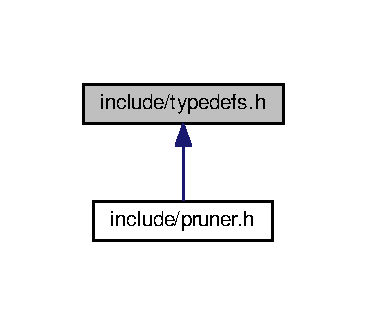
\includegraphics[width=176pt]{typedefs_8h__dep__incl}
\end{center}
\end{figure}
\subsection*{Typedefs}
\begin{DoxyCompactItemize}
\item 
typedef unsigned int \hyperlink{typedefs_8h_a91ad9478d81a7aaf2593e8d9c3d06a14}{uint}\hypertarget{typedefs_8h_a91ad9478d81a7aaf2593e8d9c3d06a14}{}\label{typedefs_8h_a91ad9478d81a7aaf2593e8d9c3d06a14}

\begin{DoxyCompactList}\small\item\em Unsigned integer. \end{DoxyCompactList}\item 
typedef std\+::vector$<$ \hyperlink{typedefs_8h_a91ad9478d81a7aaf2593e8d9c3d06a14}{uint} $>$ \hyperlink{typedefs_8h_ad56dde311aef1af823f4351451e8a381}{v\+\_\+uint}\hypertarget{typedefs_8h_ad56dde311aef1af823f4351451e8a381}{}\label{typedefs_8h_ad56dde311aef1af823f4351451e8a381}

\begin{DoxyCompactList}\small\item\em A vector of unsigned integers. \end{DoxyCompactList}\item 
typedef std\+::vector$<$ \hyperlink{typedefs_8h_ad56dde311aef1af823f4351451e8a381}{v\+\_\+uint} $>$ \hyperlink{typedefs_8h_a889a1eb698faf8cdf9160d65a20d316d}{vv\+\_\+uint}\hypertarget{typedefs_8h_a889a1eb698faf8cdf9160d65a20d316d}{}\label{typedefs_8h_a889a1eb698faf8cdf9160d65a20d316d}

\begin{DoxyCompactList}\small\item\em A vector of unsigned integer vectors. \end{DoxyCompactList}\item 
typedef std\+::vector$<$ bool $>$ \hyperlink{typedefs_8h_a15a5deffe8bbc328d6b864316ab93cea}{v\+\_\+bool}\hypertarget{typedefs_8h_a15a5deffe8bbc328d6b864316ab93cea}{}\label{typedefs_8h_a15a5deffe8bbc328d6b864316ab93cea}

\begin{DoxyCompactList}\small\item\em A vector of logicals. \end{DoxyCompactList}\item 
typedef std\+::shared\+\_\+ptr$<$ Fun\+Args $>$ \hyperlink{typedefs_8h_a36d9dc9d55255609cd5999fe2a705730}{sptr\+\_\+args}\hypertarget{typedefs_8h_a36d9dc9d55255609cd5999fe2a705730}{}\label{typedefs_8h_a36d9dc9d55255609cd5999fe2a705730}

\begin{DoxyCompactList}\small\item\em Shorthand for shared\+\_\+ptr$<$ Fun\+Args $>$ \end{DoxyCompactList}\end{DoxyCompactItemize}
\subsection*{Functions}
\begin{DoxyCompactItemize}
\item 
{\footnotesize template$<$class T $>$ }\\\hyperlink{typedefs_8h_a91ad9478d81a7aaf2593e8d9c3d06a14}{uint} {\bfseries find\+\_\+in\+\_\+vector} (const std\+::vector$<$ T $>$ $\ast$x, T value)\hypertarget{typedefs_8h_a083f13ddeb1ab069c27cc2eb131a56a6}{}\label{typedefs_8h_a083f13ddeb1ab069c27cc2eb131a56a6}

\end{DoxyCompactItemize}

\chapter{Example Documentation}
\hypertarget{00-hello-world_8cpp-example}{}\section{00-\/hello-\/world.\+cpp}
This shows how to create and print a \hyperlink{classTree}{Tree} class object.


\begin{DoxyCodeInclude}
\textcolor{preprocessor}{#include <iostream>}
\textcolor{preprocessor}{#include <vector>}
\textcolor{preprocessor}{#include "../include/pruner.hpp"}

\textcolor{keywordtype}{int} main () \{
  
  \textcolor{comment}{// Fake tree data}
  std::vector< unsigned int > source = \{0u, 0u, 1u, 2u, 3u\};
  std::vector< unsigned int > target = \{1u, 5u, 2u, 3u, 4u\};

  \textcolor{comment}{// Initialization of a tree object}
  \textcolor{keywordtype}{unsigned} \textcolor{keywordtype}{int} res;
  \hyperlink{classpruner_1_1Tree}{pruner::Tree<>} tree(source, target, res);
  
  \textcolor{comment}{// Looking at the data}
  tree.print();         
  
  
  \textcolor{keywordflow}{return} 0;
  
\}
\end{DoxyCodeInclude}
 
\hypertarget{01-adding-function_8cpp-example}{}\section{01-\/adding-\/function.\+cpp}
In this example we add a function to the tree (including a pointer to the arguments). This includes the definition of the class Tree\+Data, which is stored as args in the \hyperlink{classTree}{Tree} object.


\begin{DoxyCodeInclude}
\textcolor{preprocessor}{#include <iostream>}
\textcolor{preprocessor}{#include <vector>}
\textcolor{preprocessor}{#include "../include/pruner.h"}

\textcolor{comment}{// STEP 1: Need to declare this class}
\textcolor{keyword}{class }pruner::TreeData \{
  \textcolor{keywordtype}{int} nnodes;
\textcolor{keyword}{public}:
  
  ~TreeData() \{\};
  TreeData(\textcolor{keywordtype}{int} n): nnodes(n) \{\};
  
  \textcolor{keywordtype}{int} get\_nnodes() \{\textcolor{keywordflow}{return} this->nnodes;\};
  \textcolor{keywordtype}{void} set\_nnodes(\textcolor{keywordtype}{int} n) \{
    this->nnodes = n;
    \textcolor{keywordflow}{return};
  \};
\};

\textcolor{comment}{// STEP 2: Define a function to be passed to the algorithm}
\textcolor{keywordtype}{void} myfunction(
    \hyperlink{namespacepruner_a533476fef17527e75c4fba71d8c4ce50}{pruner::sptr\_treedata} a,
    \hyperlink{classpruner_1_1TreeIterator}{pruner::TreeIterator} & iter) \{
  
  \textcolor{comment}{// Moving a single step up}
  printf(\textcolor{stringliteral}{"Currently sitting on the node %i.\(\backslash\)nCurrent parents are: "}, iter.\hyperlink{classpruner_1_1TreeIterator_ae76ec4f2c1390d72889f78a51d65d19c}{id}());
  \textcolor{keywordflow}{for} (\textcolor{keyword}{auto} i = iter.\hyperlink{classpruner_1_1TreeIterator_a3cb8dd28630f065472e135f7db822abf}{begin\_par}(); i != iter.\hyperlink{classpruner_1_1TreeIterator_aac5656fc5b550cb8dfa4a9ebd5ea910a}{end\_par}(); ++i) \{
    printf(\textcolor{stringliteral}{" %i"}, *i);
  \}
  printf(\textcolor{stringliteral}{"\(\backslash\)n"});
  
  iter.\hyperlink{classpruner_1_1TreeIterator_adca1d999f093a69e2f5d044b358e5da7}{up}();
  printf(\textcolor{stringliteral}{"Currently sitting on the node %i.\(\backslash\)nCurrent parents are: "}, iter.\hyperlink{classpruner_1_1TreeIterator_ae76ec4f2c1390d72889f78a51d65d19c}{id}());
  \textcolor{keywordflow}{for} (\textcolor{keyword}{auto} i = iter.\hyperlink{classpruner_1_1TreeIterator_a3cb8dd28630f065472e135f7db822abf}{begin\_par}(); i != iter.\hyperlink{classpruner_1_1TreeIterator_aac5656fc5b550cb8dfa4a9ebd5ea910a}{end\_par}(); ++i) \{
    printf(\textcolor{stringliteral}{" %i"}, *i);
  \}
  printf(\textcolor{stringliteral}{"\(\backslash\)n"});
  \textcolor{keywordflow}{return};
\}

\textcolor{keywordtype}{int} main () \{
  
  \textcolor{comment}{// Fake tree data}
  \hyperlink{namespacepruner_af0145646bd7ede012cd336b416bc5579}{pruner::v\_uint} source = \{0u, 0u, 1u, 2u, 3u\};
  \hyperlink{namespacepruner_af0145646bd7ede012cd336b416bc5579}{pruner::v\_uint} target = \{1u, 5u, 2u, 3u, 4u\};
  
  \textcolor{comment}{// Initialization of a tree object}
  \hyperlink{namespacepruner_a659e6e64a9e2b8e981c3d34262a2f67e}{pruner::uint} res;
  \hyperlink{classpruner_1_1Tree}{pruner::Tree} tree(source, target, res);
  
  \textcolor{comment}{// Looking at the data}
  tree.print();         
  
  \textcolor{comment}{// We can pass the function:}
  \textcolor{comment}{// Adding function arguments}
  tree.\hyperlink{classpruner_1_1Tree_ac61a4133ceae4ea3473ea84df94f0931}{args} = std::make\_shared< pruner::TreeData >(1);
  tree.\hyperlink{classpruner_1_1Tree_a095f59358c914fb66939d2d82ca3ebc4}{fun} = myfunction;
  
  \textcolor{comment}{// Calling functions}
  tree.\hyperlink{classpruner_1_1Tree_ac61a4133ceae4ea3473ea84df94f0931}{args}->set\_nnodes(5);
  tree.\hyperlink{classpruner_1_1Tree_abaa9ef6d7eacf37302d29c12c2180c3a}{eval\_fun}();   \textcolor{comment}{// Implicit call}
  
  tree.\hyperlink{classpruner_1_1Tree_a7d465880d18acf79f3a772ea5412b0d7}{prune\_postorder}();
  
  
  \textcolor{keywordflow}{return} 0;
  
\}
\end{DoxyCodeInclude}
 
\hypertarget{02-rcpp_8cpp-example}{}\section{02-\/rcpp.\+cpp}
Shows how can this library be used within R.


\begin{DoxyCodeInclude}
\textcolor{preprocessor}{#include <Rcpp.h>}
\textcolor{preprocessor}{#include "../include/pruner.hpp"}  

\textcolor{keyword}{using namespace }Rcpp; 

\textcolor{comment}{// Users work from here on -----------------------------------------------------}

\textcolor{comment}{// Need to declare this class}
\textcolor{keyword}{class }pruner::TreeData \{
  \textcolor{keywordtype}{int} nnodes;
\textcolor{keyword}{public}:
  
  ~TreeData() \{\};
  TreeData(\textcolor{keywordtype}{int} n): nnodes(n) \{\};
  
  \textcolor{keywordtype}{int} get\_nnodes() \{\textcolor{keywordflow}{return} this->nnodes;\};
  \textcolor{keywordtype}{void} set\_nnodes(\textcolor{keywordtype}{int} n) \{
    this->nnodes = n;
    \textcolor{keywordflow}{return};
  \};
\};

\textcolor{keywordtype}{void} myfunction(
    pruner::TreeData * a,
    \hyperlink{classpruner_1_1TreeIterator}{pruner::TreeIterator} & iter
  ) \{
  
  \textcolor{comment}{// Moving a single step up}
  printf(\textcolor{stringliteral}{"Currently sitting on the node %i.\(\backslash\)nCurrent parents are: "}, iter.\hyperlink{classpruner_1_1TreeIterator_aa0d37262febc59a1b229e98ce610b30a}{id}());
  \textcolor{keywordflow}{for} (\textcolor{keyword}{auto} i = iter.\hyperlink{classpruner_1_1TreeIterator_ac401c51b2a8b33e7db63b850350c21ce}{begin\_par}(); i != iter.\hyperlink{classpruner_1_1TreeIterator_a89ccb546a2fc6add499ac54ecb5271f8}{end\_par}(); ++i) \{
    printf(\textcolor{stringliteral}{" %i"}, *i);
  \}
  printf(\textcolor{stringliteral}{"\(\backslash\)n"});
  
  iter.\hyperlink{classpruner_1_1TreeIterator_adca1d999f093a69e2f5d044b358e5da7}{up}();
  printf(\textcolor{stringliteral}{"Currently sitting on the node %i.\(\backslash\)nCurrent parents are: "}, iter.\hyperlink{classpruner_1_1TreeIterator_aa0d37262febc59a1b229e98ce610b30a}{id}());
  \textcolor{keywordflow}{for} (\textcolor{keyword}{auto} i = iter.\hyperlink{classpruner_1_1TreeIterator_ac401c51b2a8b33e7db63b850350c21ce}{begin\_par}(); i != iter.\hyperlink{classpruner_1_1TreeIterator_a89ccb546a2fc6add499ac54ecb5271f8}{end\_par}(); ++i) \{
    printf(\textcolor{stringliteral}{" %i"}, *i);
  \}
  printf(\textcolor{stringliteral}{"\(\backslash\)n"});
  \textcolor{keywordflow}{return};
\}

\textcolor{comment}{// [[Rcpp::export]]}
List fancytree(\textcolor{keyword}{const} \hyperlink{namespacepruner_af0145646bd7ede012cd336b416bc5579}{pruner::v\_uint} & parents, \textcolor{keyword}{const} 
      \hyperlink{namespacepruner_af0145646bd7ede012cd336b416bc5579}{pruner::v\_uint} & offspring) \{
  
  \textcolor{comment}{// Creating the object}
  uint ans;
  \hyperlink{classpruner_1_1Tree}{pruner::Tree} mytree(parents, offspring, ans);
  
  \textcolor{comment}{// Adding function arguments}
  mytree.\hyperlink{classpruner_1_1Tree_afe84a58af72b0d544dcc7ceff96daf8d}{args} = \textcolor{keyword}{new} pruner::TreeData(1);
  mytree.\hyperlink{classpruner_1_1Tree_a243f4077cc9974d6de6a6af0f3e9b0fd}{fun} = myfunction;
  
  \textcolor{comment}{// Calling functions}
  mytree.\hyperlink{classpruner_1_1Tree_afe84a58af72b0d544dcc7ceff96daf8d}{args}->set\_nnodes(5);
  mytree.\hyperlink{classpruner_1_1Tree_abaa9ef6d7eacf37302d29c12c2180c3a}{eval\_fun}();   \textcolor{comment}{// Implicit call}
  
  \textcolor{comment}{// Example printing}
  mytree.print();
  
  List res = List::create(
    \_[\textcolor{stringliteral}{"edgelist"}]  = mytree.get\_edgelist(),
    \_[\textcolor{stringliteral}{"postorder"}] = mytree.get\_postorder(),
    \_[\textcolor{stringliteral}{"dag"}]       = mytree.is\_dag()
  );
  
  \textcolor{keyword}{delete} mytree.\hyperlink{classpruner_1_1Tree_afe84a58af72b0d544dcc7ceff96daf8d}{args};
  mytree.\hyperlink{classpruner_1_1Tree_afe84a58af72b0d544dcc7ceff96daf8d}{args} = \textcolor{keyword}{nullptr};
  
  \textcolor{keywordflow}{return} res;
  
\}

\textcolor{comment}{/***R}
\textcolor{comment}{# set.seed(8)}
\textcolor{comment}{}
\textcolor{comment}{# Is it working?}
\textcolor{comment}{tree <-}
\textcolor{comment}{  structure(}
\textcolor{comment}{    list(}
\textcolor{comment}{      edge = structure(c(4L, 5L, 5L, 4L, 5L, 1L, 2L,}
\textcolor{comment}{                         3L), .Dim = c(4L, 2L)),}
\textcolor{comment}{      tip.label = c("t3", "t2", "t1"),}
\textcolor{comment}{      edge.length = c(}
\textcolor{comment}{        0.718927504029125,}
\textcolor{comment}{        0.290873386897147,}
\textcolor{comment}{        0.932269813260064,}
\textcolor{comment}{        0.769146954407915}
\textcolor{comment}{      ),}
\textcolor{comment}{      Nnode = 2L}
\textcolor{comment}{    ),}
\textcolor{comment}{    class = "phylo",}
\textcolor{comment}{    order = "cladewise"}
\textcolor{comment}{  )}
\textcolor{comment}{ans <- fancytree(tree$edge[,1] - 1, tree$edge[,2] - 1)}
\textcolor{comment}{}
\textcolor{comment}{# plot(tree, show.node.label = TRUE)}
\textcolor{comment}{# cbind(1:length(unlist(ans[[1]])), unlist(ans[[1]]) + 1)}
\textcolor{comment}{# }
\textcolor{comment}{# # DAGS NO DAGS}
\textcolor{comment}{# invisible(fancytree(tree$edge[,1] - 1, tree$edge[,2] - 1))}
\textcolor{comment}{# E <- tree$edge}
\textcolor{comment}{# E <- rbind(E, rev(E[3,]))}
\textcolor{comment}{# E - 1L}
\textcolor{comment}{# fancytree(E[,1] - 1, E[,2] - 1) # NOT A DAG}
\textcolor{comment}{# }
\textcolor{comment}{# library(igraph)}
\textcolor{comment}{# plot(graph\_from\_edgelist(E), vertex.label = 0:4, vertex.size = 40)}
\textcolor{comment}{}
\textcolor{comment}{*/}
\end{DoxyCodeInclude}
 
%--- End generated contents ---

% Index
\backmatter
\newpage
\phantomsection
\clearemptydoublepage
\addcontentsline{toc}{chapter}{Index}
\printindex

\end{document}
